\documentclass[border=6pt]{standalone}
\usepackage{tikz}
\usetikzlibrary{arrows.meta,positioning,calc,fit,backgrounds}

\definecolor{slate}{HTML}{334155}
\definecolor{slateLight}{HTML}{64748B}
\definecolor{panelFill}{HTML}{ECFEFF}
\definecolor{panelStroke}{HTML}{0891B2}
\definecolor{batteryFill}{HTML}{F0FDF4}
\definecolor{batteryStroke}{HTML}{16A34A}
\definecolor{loadFill}{HTML}{FFF7ED}
\definecolor{loadStroke}{HTML}{EA580C}
\definecolor{noteFill}{HTML}{F8FAFC}
\definecolor{noteStroke}{HTML}{CBD5E1}

\begin{document}
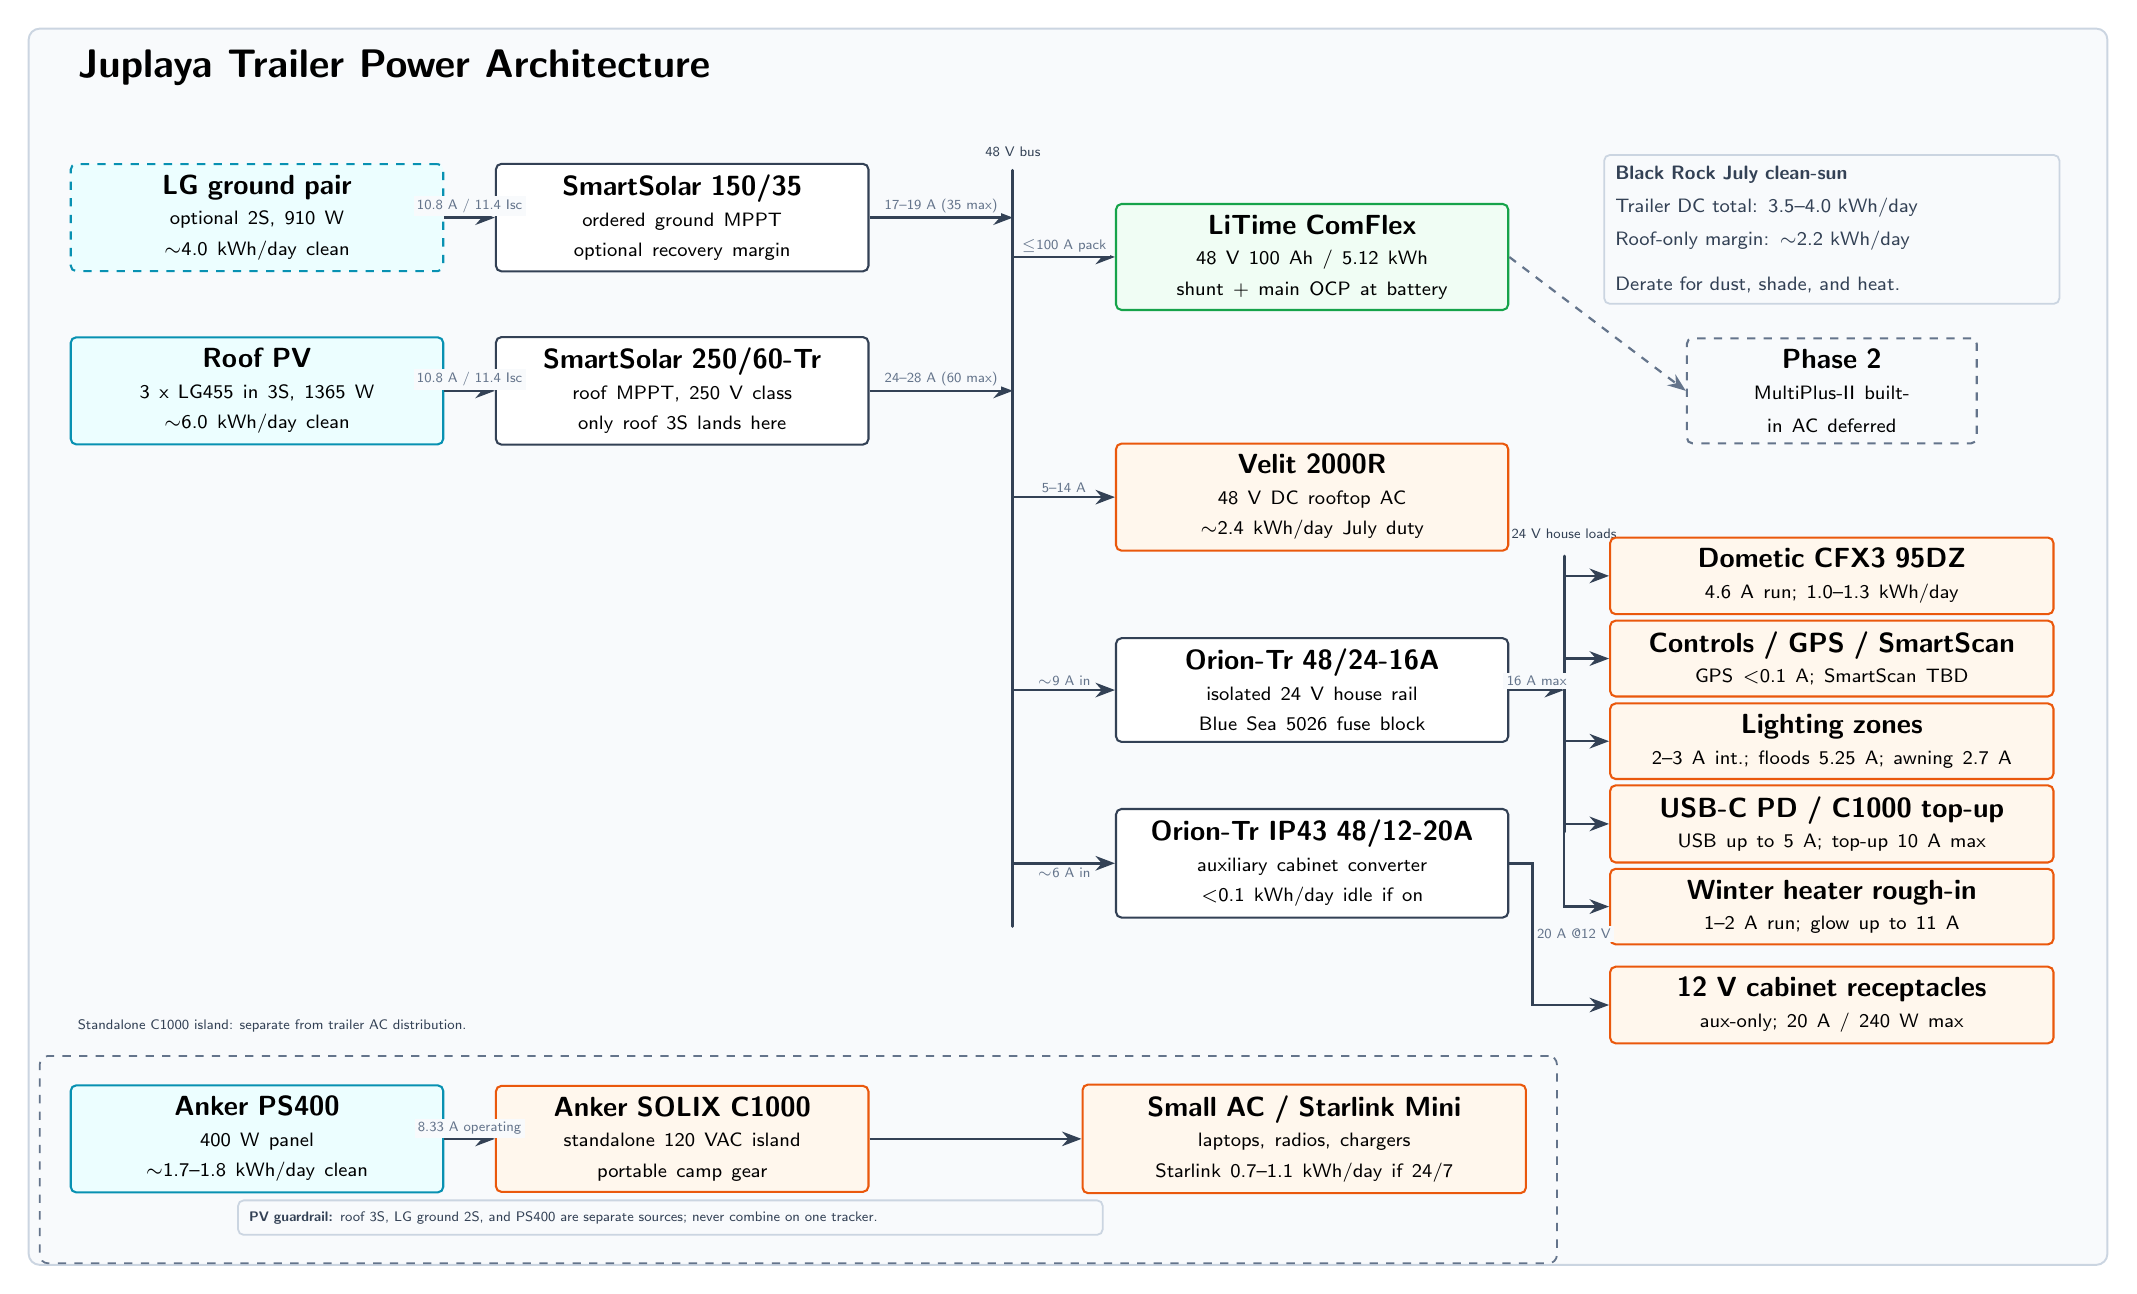
\begin{tikzpicture}[
  font=\sffamily,
  >=Stealth,
  title/.style={font=\sffamily\bfseries\Large, text=black},
  smallnote/.style={font=\sffamily\tiny, text=slate, align=left},
  block/.style={
    draw=slate,
    fill=white,
    rounded corners=2pt,
    line width=0.75pt,
    align=center,
    inner sep=4pt,
    minimum height=1.25cm
  },
  source/.style={block, fill=panelFill, draw=panelStroke},
  optionalSource/.style={source, dashed},
  battery/.style={block, fill=batteryFill, draw=batteryStroke},
  load/.style={block, fill=loadFill, draw=loadStroke},
  phase/.style={block, fill=noteFill, draw=slateLight, dashed},
  note/.style={
    draw=noteStroke,
    fill=noteFill,
    rounded corners=2pt,
    line width=0.65pt,
    align=left,
    inner sep=4pt,
    font=\sffamily\tiny,
    text=slate
  },
  leadlabel/.style={
    font=\sffamily\tiny,
    text=slateLight,
    fill=noteFill,
    inner sep=1.2pt,
    align=center
  },
  island/.style={
    draw=slateLight,
    fill=noteFill,
    rounded corners=3pt,
    dashed,
    line width=0.65pt
  },
  bus/.style={draw=slate, line width=1.1pt, line cap=round},
  arr/.style={->, draw=slate, line width=0.9pt},
  softarr/.style={->, draw=slateLight, line width=0.8pt, dashed}
]

\begin{scope}[on background layer]
  \draw[draw=noteStroke, fill=noteFill, rounded corners=4pt, line width=0.7pt]
    (-0.25,0.25) rectangle (26.15,15.95);
\end{scope}

\node[title, anchor=west] at (0.25,15.45) {Juplaya Trailer Power Architecture};

% Primary trailer PV and 48 V system.
\node[optionalSource, text width=4.45cm] (groundpv) at (2.65,13.55)
  {{\bfseries LG ground pair}\\[-1pt]
   {\scriptsize optional 2S, 910 W}\\[-1pt]
   {\scriptsize \(\sim\)4.0 kWh/day clean}};

\node[block, text width=4.45cm] (groundmppt) at (8.05,13.55)
  {{\bfseries SmartSolar 150/35}\\[-1pt]
   {\scriptsize ordered ground MPPT}\\[-1pt]
   {\scriptsize optional recovery margin}};

\node[source, text width=4.45cm] (roofpv) at (2.65,11.35)
  {{\bfseries Roof PV}\\[-1pt]
   {\scriptsize 3 x LG455 in 3S, 1365 W}\\[-1pt]
   {\scriptsize \(\sim\)6.0 kWh/day clean}};

\node[block, text width=4.45cm] (roofmppt) at (8.05,11.35)
  {{\bfseries SmartSolar 250/60-Tr}\\[-1pt]
   {\scriptsize roof MPPT, 250 V class}\\[-1pt]
   {\scriptsize only roof 3S lands here}};

\coordinate (busTop) at (12.25,14.15);
\coordinate (busBottom) at (12.25,4.55);
\coordinate (busGround) at (12.25,13.55);
\coordinate (busRoof) at (12.25,11.35);
\coordinate (busBattery) at (12.25,13.05);
\coordinate (busVelit) at (12.25,10.00);
\coordinate (busOrion24) at (12.25,7.55);
\coordinate (busOrion12) at (12.25,5.35);
\draw[bus] (busTop) -- (busBottom);
\node[smallnote, anchor=south, align=center] at (12.25,14.2) {48 V bus};

\node[battery, text width=4.7cm] (battery) at (16.05,13.05)
  {{\bfseries LiTime ComFlex}\\[-1pt]
   {\scriptsize 48 V 100 Ah / 5.12 kWh}\\[-1pt]
   {\scriptsize shunt + main OCP at battery}};

\node[load, text width=4.7cm] (velit) at (16.05,10.00)
  {{\bfseries Velit 2000R}\\[-1pt]
   {\scriptsize 48 V DC rooftop AC}\\[-1pt]
   {\scriptsize \(\sim\)2.4 kWh/day July duty}};

\node[block, text width=4.7cm] (orion24) at (16.05,7.55)
  {{\bfseries Orion-Tr 48/24-16A}\\[-1pt]
   {\scriptsize isolated 24 V house rail}\\[-1pt]
   {\scriptsize Blue Sea 5026 fuse block}};

\node[block, text width=4.7cm] (orion12) at (16.05,5.35)
  {{\bfseries Orion-Tr IP43 48/12-20A}\\[-1pt]
   {\scriptsize auxiliary cabinet converter}\\[-1pt]
   {\scriptsize \(<\)0.1 kWh/day idle if on}};

% 24 V and 12 V loads.
\coordinate (houseBusTop) at (19.25,9.25);
\coordinate (houseBusBottom) at (19.25,5.75);
\draw[bus] (houseBusTop) -- (houseBusBottom);
\node[smallnote, anchor=south, align=center] at (19.25,9.35) {24 V house loads};

\node[load, text width=5.35cm, minimum height=0.8cm] (fridge) at (22.65,9.00)
  {{\bfseries Dometic CFX3 95DZ}\\[-1pt]
   {\scriptsize 4.6 A run; 1.0--1.3 kWh/day}};

\node[load, text width=5.35cm, minimum height=0.8cm] (controls) at (22.65,7.95)
  {{\bfseries Controls / GPS / SmartScan}\\[-1pt]
   {\scriptsize GPS \(<\)0.1 A; SmartScan TBD}};

\node[load, text width=5.35cm, minimum height=0.8cm] (lights) at (22.65,6.90)
  {{\bfseries Lighting zones}\\[-1pt]
   {\scriptsize 2--3 A int.; floods 5.25 A; awning 2.7 A}};

\node[load, text width=5.35cm, minimum height=0.8cm] (usb) at (22.65,5.85)
  {{\bfseries USB-C PD / C1000 top-up}\\[-1pt]
   {\scriptsize USB up to 5 A; top-up 10 A max}};

\node[load, text width=5.35cm, minimum height=0.8cm] (heater) at (22.65,4.80)
  {{\bfseries Winter heater rough-in}\\[-1pt]
   {\scriptsize 1--2 A run; glow up to 11 A}};

\node[load, text width=5.35cm, minimum height=0.8cm] (cab12) at (22.65,3.55)
  {{\bfseries 12 V cabinet receptacles}\\[-1pt]
   {\scriptsize aux-only; 20 A / 240 W max}};

\node[phase, text width=3.4cm, minimum height=1.0cm] (phase2) at (22.65,11.35)
  {{\bfseries Phase 2}\\[-1pt]
   {\scriptsize MultiPlus-II built-in AC deferred}};

\node[note, text width=5.5cm, font=\sffamily\scriptsize, minimum height=1.75cm] (energy) at (22.65,13.40)
  {{\bfseries Black Rock July clean-sun}\\[4pt]
   Trailer DC total: 3.5--4.0 kWh/day\\[4pt]
   Roof-only margin: \(\sim\)2.2 kWh/day\\[8pt]
   Derate for dust, shade, and heat.};

\node[source, text width=4.45cm] (ps400) at (2.65,1.85)
  {{\bfseries Anker PS400}\\[-1pt]
   {\scriptsize 400 W panel}\\[-1pt]
   {\scriptsize \(\sim\)1.7--1.8 kWh/day clean}};

\node[load, text width=4.45cm] (c1000) at (8.05,1.85)
  {{\bfseries Anker SOLIX C1000}\\[-1pt]
   {\scriptsize standalone 120 VAC island}\\[-1pt]
   {\scriptsize portable camp gear}};

\node[load, text width=5.35cm] (acloads) at (15.95,1.85)
  {{\bfseries Small AC / Starlink Mini}\\[-1pt]
   {\scriptsize laptops, radios, chargers}\\[-1pt]
   {\scriptsize Starlink 0.7--1.1 kWh/day if 24/7}};

\node[smallnote, anchor=west] at (0.25,3.28)
  {Standalone C1000 island: separate from trailer AC distribution.};

\node[note, text width=10.7cm] (pvguard) at (7.90,0.85)
  {{\bfseries PV guardrail:} roof 3S, LG ground 2S, and PS400 are separate sources; never combine on one tracker.};

\begin{scope}[on background layer]
  \node[island, fit=(ps400) (c1000) (acloads) (pvguard), inner xsep=0.38cm, inner ysep=0.35cm] {};
\end{scope}

% Power-flow arrows.
\draw[arr] (groundpv.east) -- node[leadlabel, above] {10.8 A / 11.4 Isc} (groundmppt.west);
\draw[arr] (groundmppt.east) -- node[leadlabel, above] {17--19 A (35 max)} (busGround);
\draw[arr] (roofpv.east) -- node[leadlabel, above] {10.8 A / 11.4 Isc} (roofmppt.west);
\draw[arr] (roofmppt.east) -- node[leadlabel, above] {24--28 A (60 max)} (busRoof);
\draw[arr] (busBattery) -- node[leadlabel, above] {\(\le\)100 A pack} (battery.west);
\draw[arr] (busVelit) -- node[leadlabel, above] {5--14 A} (velit.west);
\draw[arr] (busOrion24) -- node[leadlabel, above] {\(\sim\)9 A in} (orion24.west);
\draw[arr] (busOrion12) -- node[leadlabel, below] {\(\sim\)6 A in} (orion12.west);
\draw[arr] (orion24.east) -- node[leadlabel, above] {16 A max} (19.25,7.55);
\draw[arr] (19.25,9.00) -- (fridge.west);
\draw[arr] (19.25,7.95) -- (controls.west);
\draw[arr] (19.25,6.90) -- (lights.west);
\draw[arr] (19.25,5.85) -- (usb.west);
\draw[arr] (19.25,5.75) |- (heater.west);
\draw[arr] (orion12.east) -- (18.85,5.35) -- node[leadlabel, right] {20 A @12 V} (18.85,3.55) -- (cab12.west);
\draw[softarr] (battery.east) -- (phase2.west);

\draw[arr] (ps400.east) -- node[leadlabel, above] {8.33 A operating} (c1000.west);
\draw[arr] (c1000.east) -- (acloads.west);

\end{tikzpicture}
\end{document}
